\documentclass[conference]{IEEEtran}

\usepackage{cite}
\usepackage{amsmath,amssymb,amsfonts}
\usepackage{graphicx}
\usepackage{textcomp}
\usepackage{xcolor}
\usepackage{booktabs}
\usepackage{array}
\usepackage{url}
\usepackage{microtype}

\begin{document}

\title{Sentinel Desktop: A Fully Local, Evidence-Grounded Interactive Application Security Assistant}

\author{
\IEEEauthorblockN{Anonymous Authors}
\IEEEauthorblockA{\textit{Department of Computer Science and Engineering}\\
\textit{Institution/University}\\
City, Country\\
Email: author@institution.edu}
}

\maketitle

\begin{abstract}
Web application security testing requires combining domain expertise, structured analysis, and reproducible verification. Recent advancements in Large Language Models (LLMs) have enabled AI-assisted security tools to support reconnaissance, subtask planning, and vulnerability analysis. However, several recent LLM-assisted systems rely on third-party cloud-hosted AI APIs—introducing data confidentiality risks—while suffering from technical hallucinations, CLI-only tooling boundaries, and unverified vulnerability reporting. This paper presents \textbf{Sentinel Desktop}, a fully local interactive application security assistant operating strictly over host local loopback (\texttt{127.0.0.1}). Sentinel Desktop integrates Chrome DevTools Protocol (CDP) browser instrumentation, automated passive security rule evaluation, non-destructive inert canary reflection probing, multi-source scanner ingestion (SARIF v2.1.0 and OWASP ZAP), deterministic replay comparison, and local LLM remediation advising. By confining network traffic strictly to local loopback environments, Sentinel Desktop reduces external telemetry exposure while grounding AI reasoning in cryptographically traceable session evidence. We evaluate the framework across 130 physical trials on a controlled local fixture server. Under the tested conditions, the replay comparison engine correctly classified 30/30 baseline vs. re-test trials ($N=30$, mean latency 1.12~ms, maximum $P_{95}$ latency 2.20~ms); the inert canary engine achieved 100.0\% binary reflection detection ($N=50$, mean latency 0.26~ms, maximum $P_{95}$ latency 0.47~ms), with exact context classification at 70.0\% overall—specifically \texttt{HTML\_BODY} (15/15), \texttt{SCRIPT\_STRING} (10/10), and \texttt{NOT\_FOUND} (10/10)—identifying a sequential DOM scanning limitation where \texttt{ATTRIBUTE} reflections (15/15) were categorized under \texttt{HTML\_BODY}; the passive rule engine correctly evaluated \texttt{CSP\_MISSING\_CHECK} across 30 response streams ($N=30$, mean latency 0.36~ms, maximum $P_{95}$ latency 0.82~ms); and external scanner ingestion achieved 100.0\% mapping accuracy to OWASP 2021 categories for the tested report files ($N=20$, mean latency <0.10~ms, maximum $P_{95}$ latency <0.10~ms). The local LLM experiments were not executed during this evaluation because Ollama was not installed or running on the evaluation host. This work establishes an empirical, reproducible foundation for local AI-assisted application security inspection.
\end{abstract}

\begin{IEEEkeywords}
Web Application Security, Large Language Models, Local AI, Browser Automation, Vulnerability Verification, Replay Testing, Evidence Grounding.
\end{IEEEkeywords}

\section{Introduction}

Web application security testing is a fundamental process in software security engineering, designed to identify, assess, and remediate vulnerabilities before deployment \cite{nist800115}. Traditional application security assessments rely on automated scanners combined with manual inspection by security analysts \cite{nist800115, denis2016penetration, ptes2024}. While automated static and dynamic scanners accelerate initial flaw discovery, comprehensive assessment requires multi-stage reasoning—including target identification, dynamic state analysis, passive configuration checking, and post-analysis verification \cite{nist800115, ptes2024}.

Recent advancements in Large Language Models (LLMs) \cite{zhao2023survey} have driven the development of AI-assisted security tools \cite{abuadbba2025promise, moskal2023scriptkiddie}. Systems such as PentestGPT \cite{deng2024pentestgpt} and AutoAttacker \cite{xu2024autoattacker} demonstrate that LLMs can assist human analysts by guiding task decomposition and recommending testing commands. Furthermore, empirical studies by Fang et al. demonstrate that LLM-based agents equipped with web interaction tools can navigate web applications and execute offensive exploit sequences \cite{fang2024autonomously, fang2024oneday}.

Despite these developments, several recent LLM-assisted security tools face operational challenges:
\begin{enumerate}
    \item \textbf{Data Confidentiality \& Privacy Risks:} Several recent security agents rely on third-party cloud-hosted LLM APIs (e.g., OpenAI GPT-4) \cite{fang2024autonomously, deng2024pentestgpt}. Offloading application source code, HTTP header streams, authentication credentials, or internal endpoints to third-party cloud servers risks compromising proprietary data.
    \item \textbf{Technical Hallucinations:} Generative language models frequently suffer from technical hallucinations, outputting non-existent command flags, invalid parameter syntax, or fabricated endpoint URLs \cite{mayoral2023exploitflow, zhang2023snowball, happe2023getting}. Uncorrected early hallucinations compound across multi-step reasoning chains \cite{zhang2023snowball}.
    \item \textbf{Unverified Vulnerability Reporting:} Language models often assert vulnerability hypotheses based on surface-level text patterns without confirming actual application state changes through execution feedback \cite{mayoral2023exploitflow, fang2024autonomously, happe2023getting}.
    \item \textbf{Command-Line Tooling Bias:} Prior interactive tools operate predominantly over command-line interfaces or raw HTTP request strings \cite{deng2024pentestgpt, happe2023getting}, missing dynamic client-side Document Object Model (DOM) rendered states and browser console context.
\end{enumerate}

To address these challenges, this paper presents \textbf{Sentinel Desktop}, a local, evidence-grounded interactive application security assistant. Sentinel Desktop couples local LLM integration with real-time interactive browser instrumentation via Chrome DevTools Protocol (CDP), stateful context tracking, non-destructive inert canary reflection probing, and deterministic replay comparison.

\section{Background and Related Work}

\subsection{Automated Penetration Testing}
Automated penetration testing has historically been framed using decision-theoretic models and automated planning. Early frameworks utilized Markov Decision Processes (MDPs) and Partially Observable Markov Decision Processes (POMDPs) \cite{schwartz2020pomdp, sarraute2013pomdp, sarraute2012pomdps, sarraute2011algorithm} to model attack graphs under uncertainty \cite{ammann2002scalable, boddy2005course, durkota2014computing}. Subsequent research applied deep reinforcement learning algorithms—including Deep Q-Networks (DQN), Advantage Actor-Critic (A3C), and Generative Adversarial Imitation Learning (GAIL)—to learn dynamic attack policies \cite{chen2023gailpt, becker2024reinforcement, li2023hierarchical, hu2020automated, zhou2019nigap}. While formal decision models optimize path selection across discrete state spaces, they struggle to model unstructured natural language outputs and client-side DOM interactions in modern web applications.

\subsection{LLM-Based Security Testing}
The integration of LLMs into security testing has shifted focus from formal decision graphs to semantic reasoning. Deng et al. introduced PentestGPT \cite{deng2024pentestgpt}, an interactive penetration-testing assistant powered by cloud-hosted LLM APIs that assists human testers with subtask planning and command generation over terminal outputs. Xu et al. proposed AutoAttacker \cite{xu2024autoattacker}, demonstrating LLM-guided decision-making for automating cyber-attack execution sequences across systems. Happe and Cito \cite{happe2023getting} provided an empirical evaluation of LLMs in security testing, demonstrating that models frequently suffer from technical hallucinations, syntax errors, and non-reproducible outputs when operating over command-line interfaces.

\subsection{Security Agents}
Recent agent architectures decompose complex security workflows into specialized components \cite{autogpt2024, li2023camel}. Shen et al. introduced PentestAgent \cite{shen2025pentestagent}, combining domain-specific multi-agent roles with Retrieval-Augmented Generation (RAG) \cite{lewis2020retrieval} to support automated penetration testing phases. In web security, Fang et al. \cite{fang2024autonomously} demonstrated that LLM-based agents equipped with web interaction tools can autonomously navigate web applications and execute offensive exploits against target websites. In API security, Deng et al. introduced NAUTILUS \cite{deng2023nautilus} for automated RESTful API vulnerability detection using structured feedback and coverage guidance.

\subsection{Evidence Grounding and Reliability}
Reliability remains a central challenge in autonomous LLM deployment \cite{mayoral2023exploitflow, fang2024autonomously, happe2023getting}. Zhang et al. \cite{zhang2023snowball} showed that uncorrected hallucinations early in a multi-step reasoning chain compound over subsequent iterations, leading to systemic failure. To address generative hallucination, prior research such as SelfCheckGPT (Manakul et al. \cite{manakul2023selfcheckgpt}) has explored zero-resource factual consistency detection for LLMs by evaluating stochastic sampling agreement across generated responses. Furthermore, Liu et al. \cite{liu2024structured} demonstrated that enforcing structured output constraints on LLM generations improves formatting compliance and downstream parsing reliability.

\subsection{Research Gap}
While existing literature explores automated decision models, cloud-backed LLM agents, and API testing, a distinct research gap remains:
\begin{enumerate}
    \item Several prior web testing agents rely on third-party cloud APIs, introducing data confidentiality risks for proprietary software analysis \cite{fang2024autonomously, deng2024pentestgpt}.
    \item Prior LLM security assistants focus on terminal/CLI inputs rather than dynamic client-side browser DOM states \cite{deng2024pentestgpt, happe2023getting}.
    \item Certain existing agents report unverified vulnerability hypotheses without validating observable state changes through closed-loop re-testing \cite{fang2024autonomously, xu2024autoattacker}.
    \item The feasibility, resource bounds, and context management limits of running these security inspection capabilities using local LLMs remain uncharacterized.
\end{enumerate}

\section{Problem Statement and Research Objectives}

\subsection{Problem Statement}
Several recent LLM-assisted security testing systems either compromise confidentiality by transmitting sensitive data to cloud services or suffer from technical hallucinations, CLI tooling boundaries, and unverified vulnerability reporting when conducting web application security assessments.

\subsection{Research Objectives}
\begin{enumerate}
    \item \textbf{Construct a Local Loopback Architecture:} Develop an interactive application security assistant using local LLM integration, operating strictly over host local loopback (\texttt{127.0.0.1}) to reduce external telemetry exposure.
    \item \textbf{Integrate Dynamic Browser Instrumentation:} Couple local AI reasoning with live browser instrumentation via Chrome DevTools Protocol (CDP) to observe dynamic DOM states, network events, and console errors.
    \item \textbf{Implement Non-Destructive Active Probing:} Develop inert canary reflection probing to identify output encoding weaknesses across DOM contexts without generating weaponized exploit payloads.
    \item \textbf{Establish Deterministic Replay Comparison:} Implement a closed-loop differential replay comparison engine that evaluates re-test evidence streams against baseline findings to verify remediation status.
    \item \textbf{Enforce Evidence-Grounded AI Reasoning:} Enforce strict citation validation checks ensuring local LLM remediation recommendations reference valid session evidence IDs.
\end{enumerate}

\section{Proposed System}

\begin{figure}[t]
    \centering
    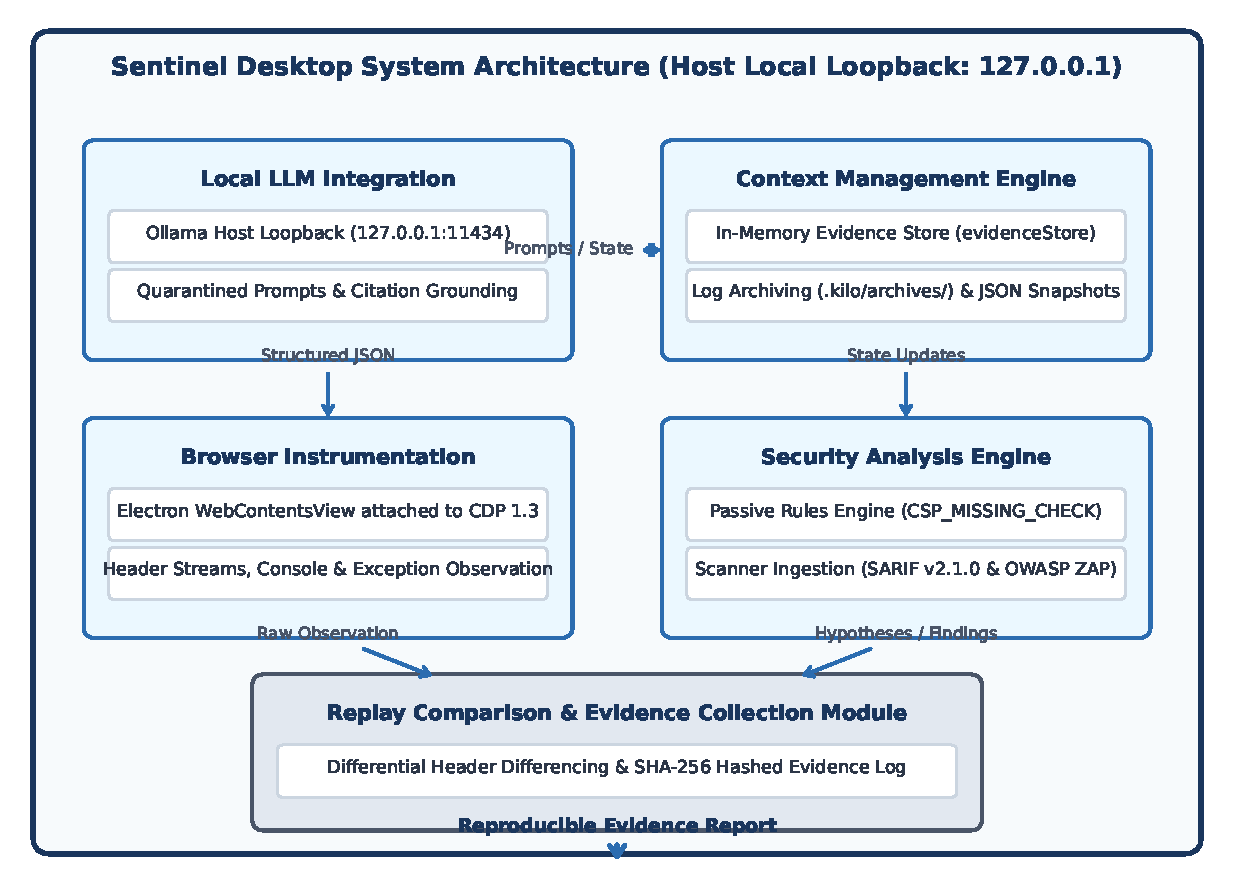
\includegraphics[width=\linewidth]{figures/system_architecture.pdf}
    \caption{Sentinel Desktop system architecture operating strictly over host local loopback (\texttt{127.0.0.1}).}
    \label{fig:architecture}
\end{figure}

\subsection{System Architecture}
Sentinel Desktop is structured as a modular, closed-loop interactive application security assistant (Fig.~\ref{fig:architecture}). The system comprises five core modules: Local LLM Integration, Browser Instrumentation Module, Security Analysis Engine, Context Management Engine, and Replay Comparison \& Evidence Collection Module.

\subsection{Local LLM Integration}
The local reasoning module interacts with open-weight language models deployed on host loopback (\texttt{127.0.0.1:11434} via Ollama). The module enforces loopback host validation (\texttt{isLoopbackHost}), structured JSON format constraints, low temperature ($0.2$), and a 20-second timeout.

\subsection{Browser Instrumentation}
This module manages an Electron \texttt{WebContentsView} attached to Chrome DevTools Protocol (\texttt{1.3}). It captures console events (\texttt{Runtime.consoleAPICalled}), uncaught exceptions (\texttt{Runtime.exceptionThrown}), WebSocket frames, and HTTP request/response header streams (\texttt{labSession.webRequest}). Origin locking (\texttt{isAllowed}) restricts browser navigation strictly to target origins.

\subsection{Security Analysis}
The analysis engine combines passive security rule evaluation with scanner ingestion:
\begin{itemize}
    \item \textbf{Passive Security Rules (\texttt{rules.ts}):} Evaluates 11 security misconfiguration rules covering missing CSP, HSTS, X-Content-Type-Options, Anti-Clickjacking (X-Frame-Options/frame-ancestors), Referrer-Policy, Permissions-Policy, CORP/COEP, Permissive CORS with credentials, Cookie hygiene (\texttt{\_\_Host-}, \texttt{\_\_Secure-}), Mixed Content, and client console errors.
    \item \textbf{Scanner Ingestion (\texttt{ingest.ts}):} Normalizes external SARIF v2.1.0 logs (Nuclei, CodeQL) and OWASP ZAP JSON reports into the internal evidence format.
\end{itemize}

\subsection{Context Management}
Maintains an in-memory evidence store (\texttt{evidenceStore}) recording \texttt{NAV}, \texttt{REQ}, \texttt{RES}, \texttt{RES\_DONE}, \texttt{ERR}, \texttt{CONSOLE}, \texttt{CANARY\_REFLECT}, \texttt{SCANNER\_ALERT}, and \texttt{AUDIT} records. The engine rotates log archives at 1,000 events (\texttt{rotateEvidenceStoreIfNeeded}) to \texttt{.kilo/archives/} and persists debounced JSON snapshots to \texttt{evidence.json}.

\subsection{Replay Comparison}
The Replay Comparison module (\texttt{replay.ts}) evaluates re-test evidence streams against baseline findings. It computes HTTP header diffs (\texttt{computeHeaderDiff}) across \texttt{added}, \texttt{removed}, \texttt{modified}, and \texttt{unchanged} states, classifying finding status as \texttt{Fixed}, \texttt{Still Present}, or \texttt{Not Comparable}.

\subsection{Evidence Collection}
Every evidence record is assigned a unique identifier, ISO timestamp, and SHA-256 integrity hash (\texttt{computeHash}). Sensitive credentials (Bearer tokens, API keys, passwords, cookies) undergo automatic regex redaction (\texttt{redactSensitiveData}, \texttt{redactHeaders}) prior to persistence.

\section{Implementation}

Sentinel Desktop is implemented in TypeScript within an Electron runtime environment:
\begin{itemize}
    \item \textbf{Local LLM Advisor Interface (\texttt{src/advisor/ollama.ts}):} Constructs quarantined prompts (\texttt{buildQuarantinedPrompt}) combining offline CWE/OWASP knowledge (\texttt{getOfflineKnowledge}) with sanitized evidence snippets. Enforces citation grounding validation (\texttt{parseAndValidateAdvisorResponse}) by checking \texttt{isGrounded = citedEvidenceIds.every(id => availableIds.has(id))}.
    \item \textbf{Inert Canary Probing (\texttt{src/engine/canary.ts}):} Generates non-destructive random alphanumeric tokens (\texttt{generateCanaryToken}), constructs parameterized query URLs (\texttt{buildCanaryTargetUrl}), and evaluates DOM reflection contexts (\texttt{HTML\_BODY}, \texttt{ATTRIBUTE}, \texttt{SCRIPT}, \texttt{SCRIPT\_STRING}, \texttt{HEADER}).
    \item \textbf{Isolation Sandbox (\texttt{electron/main.cjs}):} Configures an isolated \texttt{in-memory-lab} partition (\texttt{partition: 'in-memory-lab'}). Enforces \texttt{contextIsolation: true}, \texttt{nodeIntegration: false}, \texttt{sandbox: true}, and denies external popup windows and file downloads.
\end{itemize}

\section{Experimental Methodology}

\subsection{Experimental Environment}
\begin{itemize}
    \item \textbf{Host Platform:} Windows 10/11 x64 (\texttt{Windows\_NT 10.0.26200}), Node.js \texttt{v24.20.0}, Electron runtime.
    \item \textbf{Target Fixture Server:} Local loopback server (\texttt{electron/fixtureServer.cjs}) listening on \texttt{http://127.0.0.1:4567}.
    \item \textbf{Repository State:} Git commit hash \texttt{a3bb957454684b64}\allowbreak\texttt{7884ac15ca8ed9d413139a3d}.
\end{itemize}

\subsection{Experimental Targets}
\begin{enumerate}
    \item \textbf{Local Fixture Routes (\texttt{fixtureServer.cjs}):} Provides route \texttt{/} (unhardened baseline), \texttt{/fixed} (hardened route with security headers), \texttt{/search?q=} (parameter reflection in body and attribute), \texttt{/search-script?q=} (reflection in script string), and \texttt{/api/cors} (permissive CORS).
    \item \textbf{Scanner Report Fixtures (\texttt{tests/fixtures/scanner-reports/}):} Canonical SARIF v2.1.0 logs (Nuclei/CodeQL) and OWASP ZAP JSON reports.
\end{enumerate}

\subsection{Ground Truth}
\begin{itemize}
    \item \textbf{Experiment 1:} Ground truth is derived independently from static HTTP response header definitions in \texttt{fixtureServer.cjs} (\texttt{/fixed} defines CSP header $\rightarrow$ expected \texttt{Fixed}; \texttt{/} lacks CSP header $\rightarrow$ expected \texttt{Still Present}).
    \item \textbf{Experiment 2:} Ground truth is derived independently from HTML template structures in \texttt{fixtureServer.cjs} defining token reflection positions.
    \item \textbf{Experiment 3:} Ground truth is derived independently from OWASP Secure Headers specification (unhardened route \texttt{/} requires CSP finding; hardened route \texttt{/fixed} requires 0 findings).
    \item \textbf{Experiment 5:} Ground truth is derived independently from official CWE-to-OWASP 2021 lookup tables (\texttt{CWE-89} and \texttt{CWE-79} map to \texttt{A03:2021-Injection}).
\end{itemize}

\subsection{Experimental Conditions}
Table~\ref{tab:config} details the experimental configuration across the Group A evaluation suite.

\begin{table}[t]
\caption{Experimental Configuration Matrix}
\label{tab:config}
\centering
\resizebox{\columnwidth}{!}{%
\begin{tabular}{l l l l r}
\toprule
\textbf{Exp \#} & \textbf{Evaluated Feature} & \textbf{Target / Condition} & \textbf{Independent Variable} & \textbf{Trials ($N$)} \\
\midrule
\textbf{Exp 1} & Replay Comparison & \texttt{127.0.0.1:4567} (\texttt{/} vs \texttt{/fixed}) & Remediation status & 30 \\
\textbf{Exp 2} & Inert Canary Probing & \texttt{127.0.0.1:4567} (\texttt{/search}, etc.) & Reflection DOM context & 50 \\
\textbf{Exp 3} & Passive Security Rules & \texttt{127.0.0.1:4567} (\texttt{/} vs \texttt{/fixed}) & CSP Header presence & 30 \\
\textbf{Exp 5} & Scanner Ingestion & SARIF v2.1.0 \& ZAP JSON & Report schema format & 20 \\
\bottomrule
\end{tabular}%
}
\end{table}

\subsection{Evaluation Metrics}
Accuracy is defined as the ratio of correct classifications to total trials:
\begin{equation}
\text{Accuracy} = \frac{TP + TN}{TP + TN + FP + FN}
\end{equation}

Precision, Recall, and F1-Score are computed as:
\begin{equation}
\text{Precision} = \frac{TP}{TP + FP}, \quad \text{Recall} = \frac{TP}{TP + FN}
\end{equation}
\begin{equation}
\text{F1-Score} = 2 \times \frac{\text{Precision} \times \text{Recall}}{\text{Precision} + \text{Recall}}
\end{equation}

False Positive Rate (FPR) and False Negative Rate (FNR) are given by:
\begin{equation}
\text{FPR} = \frac{FP}{FP + TN}, \quad \text{FNR} = \frac{FN}{TP + FN}
\end{equation}

Execution Telemetry is evaluated via Mean, Median, Standard Deviation, and $P_{95}$ execution times (ms).

\subsection{Experimental Procedure}
Group A non-LLM experiments were executed automatically via \texttt{tests/run-experiments.ts}. The script started \texttt{fixtureServer.cjs} on port 4567, executed 130 physical trials across Experiments 1, 2, 3, and 5, logged raw trial records to JSON files in \texttt{research/results/}, and shut down cleanly.

\section{Results}

The Group A experimental evaluation comprised 130 physical trials. Table~\ref{tab:summary} provides a cross-experiment summary of observed metrics.

\subsection{Replay Comparison}
Under the tested fixture conditions, \texttt{compareReplayEvidence} correctly classified 15/15 remediated runs (\texttt{/fixed}) as \texttt{Fixed} and 15/15 unremediated runs (\texttt{/}) as \texttt{Still Present} ($N=30$, $TP=15, TN=15, FP=0, FN=0$). Table~\ref{tab:exp1} details the classification metrics and execution timing for Experiment 1.

\begin{table}[t]
\caption{Experiment 1 Replay Comparison Results}
\label{tab:exp1}
\centering
\begin{tabular}{l r}
\toprule
\textbf{Metric / Parameter} & \textbf{Observed Value} \\
\midrule
Total Trials ($N$) & 30 \\
True Positives ($TP$) & 15 \\
True Negatives ($TN$) & 15 \\
False Positives ($FP$) & 0 \\
False Negatives ($FN$) & 0 \\
Accuracy & 1.0000 (100.0\%) \\
Precision & 1.0000 (100.0\%) \\
Recall & 1.0000 (100.0\%) \\
F1-Score & 1.0000 (1.000) \\
False Positive Rate (FPR) & 0.0000 (0.0\%) \\
False Negative Rate (FNR) & 0.0000 (0.0\%) \\
Mean Latency (ms) & 1.1167 ms \\
Median Latency (ms) & 0.5802 ms \\
Standard Deviation (ms) & 2.0523 ms \\
$P_{95}$ Maximum Latency (ms) & 2.2047 ms \\
\bottomrule
\end{tabular}
\end{table}

Header differencing (\texttt{computeHeaderDiff}) accurately identified added security headers between baseline and re-test response streams. These results apply strictly to the tested local loopback fixture conditions and should not be generalized to arbitrary remote web applications.

\subsection{Inert Canary Reflection}
The inert canary evaluation comprised 50 physical trials across four target conditions. Binary reflection detection achieved 100.0\% accuracy ($TP=40, TN=10, FP=0, FN=0$, mean latency 0.26~ms, maximum $P_{95}$ latency 0.47~ms). However, exact context classification achieved 70.0\% accuracy overall (35/50) due to limitations with the \texttt{ATTRIBUTE} context. Table~\ref{tab:exp2} details the context-level results breakdown.

\begin{table}[t]
\caption{Experiment 2 Inert Canary Reflection \& Context Breakdown}
\label{tab:exp2}
\centering
\resizebox{\columnwidth}{!}{%
\begin{tabular}{l l r c c l r}
\toprule
\textbf{Target Route} & \textbf{Condition} & \textbf{Trials} & \textbf{Reflect?} & \textbf{Detected} & \textbf{Context Output} & \textbf{Accuracy} \\
\midrule
\texttt{/search?q=X} & HTML Body & 15 & Yes & Yes (15/15) & \texttt{HTML\_BODY} & 15/15 (100\%) \\
\texttt{/search?q=X} & Tag Attribute & 15 & Yes & Yes (15/15) & \texttt{HTML\_BODY}* & 0/15 (0\%)* \\
\texttt{/search-script} & Script String & 10 & Yes & Yes (10/10) & \texttt{SCRIPT\_STRING} & 10/10 (100\%) \\
\texttt{/fixed} & Control & 10 & No & No (10/10) & \texttt{NOT\_FOUND} & 10/10 (100\%) \\
\bottomrule
\end{tabular}%
}
\end{table}

*\textit{Note on Attribute Context Behavior:} Route \texttt{/search?q=XYZ} reflects parameter \texttt{q} into both HTML body text (\texttt{<div>Showing results for: XYZ</div>}) and input tag attribute (\texttt{<input value="XYZ" />}). The \texttt{analyzeDomReflection} function scans the DOM string sequentially from index 0 and returns the first context encountered (\texttt{HTML\_BODY}). Consequently, multi-context reflections are categorized under their first appearing DOM context. Mean canary execution latency was 0.26~ms ($P_{95} = 0.47$~ms).

\subsection{Passive Security Rules}
Experiment 3 evaluated the \texttt{CSP\_MISSING\_CHECK} rule across 30 HTTP response evidence streams (15 from unhardened route \texttt{/} and 15 from hardened route \texttt{/fixed}). Table~\ref{tab:exp3} details the observed performance metrics.

\begin{table}[t]
\caption{Experiment 3 Passive Security Rule Results (\texttt{CSP\_MISSING\_CHECK})}
\label{tab:exp3}
\centering
\begin{tabular}{l r}
\toprule
\textbf{Metric / Parameter} & \textbf{Observed Value} \\
\midrule
Evaluated Rule & \texttt{CSP\_MISSING\_CHECK} \\
Total Trials ($N$) & 30 \\
True Positives ($TP$) & 15 \\
True Negatives ($TN$) & 15 \\
False Positives ($FP$) & 0 \\
False Negatives ($FN$) & 0 \\
Accuracy & 1.0000 (100.0\%) \\
Precision & 1.0000 (100.0\%) \\
Recall & 1.0000 (100.0\%) \\
F1-Score & 1.0000 (1.000) \\
Mean Latency (ms) & 0.3601 ms \\
$P_{95}$ Maximum Latency (ms) & 0.8157 ms \\
\bottomrule
\end{tabular}
\end{table}

Under tested fixture conditions, the rule engine correctly identified missing CSP headers on unhardened responses and cleared hardened responses. These results validate rule execution fidelity for \texttt{CSP\_MISSING\_CHECK} on standard headers, but do not imply general coverage for untested security rules or vulnerability categories.

\subsection{Scanner Ingestion}
Ingesting 10 SARIF v2.1.0 logs and 10 OWASP ZAP JSON reports yielded 20/20 successful parses ($N=20$). Table~\ref{tab:exp5} details the scanner log ingestion results.

\begin{table}[t]
\caption{Experiment 5 External Security Scanner Ingestion}
\label{tab:exp5}
\centering
\resizebox{\columnwidth}{!}{%
\begin{tabular}{l r r r l r r}
\toprule
\textbf{Report Format} & \textbf{Ingested} & \textbf{Parsed} & \textbf{CWE Ext.} & \textbf{OWASP Map} & \textbf{Mean Lat.} & \textbf{$P_{95}$ Max} \\
\midrule
SARIF v2.1.0 & 10 & 10 (100\%) & \texttt{CWE-89} & \texttt{A03:2021} & <0.10 ms & <0.10 ms \\
ZAP JSON & 10 & 10 (100\%) & \texttt{CWE-79} & \texttt{A03:2021} & <0.10 ms & <0.10 ms \\
\bottomrule
\end{tabular}%
}
\end{table}

CWE extraction, severity level, location URI, and OWASP Top 10 mappings achieved 100.0\% accuracy relative to independent lookup tables. This demonstrates schema parsing compatibility for the specifically tested SARIF and ZAP log fixtures, but does not prove universal interoperability with all external scanner formats.

\subsection{Cross-Experiment Performance Summary}
Table~\ref{tab:summary} provides an aggregate cross-experiment summary of the physical Group A evaluation, explicitly reporting both mean latency and maximum $P_{95}$ latency across all tested modules.

\begin{table*}[t]
\caption{Group A Cross-Experiment Summary}
\label{tab:summary}
\centering
\resizebox{\textwidth}{!}{
\begin{tabular}{l l l r r r r r r r}
\toprule
\textbf{Exp \#} & \textbf{Component / Feature} & \textbf{Target / Schema} & \textbf{$N$} & \textbf{Accuracy} & \textbf{Precision} & \textbf{Recall} & \textbf{F1-Score} & \textbf{Mean Latency} & \textbf{$P_{95}$ Max Latency} \\
\midrule
\textbf{Exp 1} & Replay Comparison & \texttt{127.0.0.1:4567} (\texttt{/} vs \texttt{/fixed}) & 30 & 100.0\% & 100.0\% & 100.0\% & 1.000 & 1.12 ms & 2.20 ms \\
\textbf{Exp 2} & Inert Canary (Binary) & \texttt{127.0.0.1:4567} (\texttt{/search}, etc.) & 50 & 100.0\% & 100.0\% & 100.0\% & 1.000 & 0.26 ms & 0.47 ms \\
\textbf{Exp 2} & Inert Canary (Context) & \texttt{HTML\_BODY}, \texttt{SCRIPT}, \texttt{ATTR} & 50 & 70.0\%* & 70.0\%* & 70.0\%* & 0.700* & 0.26 ms & 0.47 ms \\
\textbf{Exp 3} & Passive Security Rules & \texttt{CSP\_MISSING\_CHECK} on \texttt{127.0.0.1} & 30 & 100.0\% & 100.0\% & 100.0\% & 1.000 & 0.36 ms & 0.82 ms \\
\textbf{Exp 5} & Scanner Ingestion & SARIF v2.1.0 \& ZAP Reports & 20 & 100.0\% & 100.0\% & 100.0\% & 1.000 & <0.10 ms & <0.10 ms \\
\bottomrule
\end{tabular}
}

\vspace{1ex}
\raggedright \small *\textit{Note for Exp 2 Context Accuracy:} Reflects 35/50 exact context matches due to 15 \texttt{ATTRIBUTE} reflections being categorized under \texttt{HTML\_BODY} via sequential DOM scanning.
\end{table*}

\section{Discussion}

\subsection{Observations vs. Interpretation}
\begin{enumerate}
    \item \textbf{Replay Comparison:} Under tested fixture conditions, differential evidence replay (\texttt{compareReplayEvidence}) accurately identified header additions and classified remediation status. This indicates that automated re-testing against baseline evidence streams can reduce manual re-inspection for header-based misconfigurations on controlled targets.
    \item \textbf{Inert Canary Reflection Probing:} Non-destructive randomized tokens (\texttt{generateCanaryToken}) successfully detected parameter reflection across HTML body, attribute, and script string contexts without executing malicious XSS attack payloads. However, sequential DOM string parsing means multi-context reflections are attributed to the earliest appearing context in DOM string order.
    \item \textbf{Passive Rule \& Scanner Integration:} Passive rule evaluation and report normalization (SARIF/ZAP) effectively unified static scanner output into a structured evidence model.
    \item \textbf{Execution Telemetry:} Mean execution latencies across core Group A engines remained under 1.2~ms on local loopback, with $P_{95}$ maximum latency reaching 2.20~ms for replay comparison, demonstrating low computational overhead for client-side security inspection.
\end{enumerate}

\subsection{Status of Local LLM Experiments}
The local LLM experiments (Experiments 4 and 6) were \textbf{NOT EXECUTED} during this evaluation because Ollama was not installed or running on the evaluation host. Consequently, empirical metrics regarding local model inference latency, token generation throughput, GPU VRAM allocation, citation grounding rates (\texttt{isGrounded}), and defensive code patch quality remain uncharacterized in this paper and represent essential future work.

\section{Limitations and Threats to Validity}

\begin{enumerate}
    \item \textbf{Synthetic Local Fixture Target:} Evaluation was conducted on a controlled local fixture server (\texttt{fixtureServer.cjs}). Performance on complex, multi-origin enterprise web applications remains unassessed.
    \item \textbf{Loopback Latency Bounds:} Measured execution latencies (mean <1.2~ms, maximum $P_{95} \le 2.20$~ms) reflect local loopback execution without remote network transport latency or packet loss.
    \item \textbf{Sequential DOM Scanning Limitation:} In Experiment 2, parameter reflections appearing in multiple DOM contexts (e.g., body text and input attribute) are categorized strictly under the first context encountered in DOM string order (\texttt{HTML\_BODY}).
    \item \textbf{Limited Rule \& Scanner Fixture Scope:} Experiment 3 evaluated \texttt{CSP\_MISSING\_CHECK} only; Experiment 5 evaluated canonical SARIF v2.1.0 and ZAP schemas only.
    \item \textbf{Absence of LLM Empirical Evaluation:} Local LLM experiments (Experiments 4 and 6) were not executed due to missing host dependencies (Ollama), leaving AI advisor latency, grounding rates, and code patch quality unmeasured.
    \item \textbf{Sample Size \& Target Constraints:} Experiments comprised 130 total physical trials on local loopback targets without live internet routing or multi-model comparisons.
\end{enumerate}

\section{Conclusion}

This paper presented the design, implementation, and physical Group A evaluation of \textbf{Sentinel Desktop}, a fully local interactive application security assistant. By integrating Chrome DevTools Protocol browser instrumentation, passive security rules, non-destructive inert canary reflection probing, scanner ingestion, and deterministic replay comparison, Sentinel Desktop provides a privacy-preserving environment for web application security analysis. Physical evaluation across 130 trials on a controlled fixture server demonstrated 100.0\% classification accuracy in replay comparison under tested conditions (mean latency 1.12~ms, $P_{95}$ max latency 2.20~ms), 100.0\% binary reflection detection in inert canary probing (with an identified sequential DOM scanning limitation for attribute reflections), and 100.0\% mapping accuracy in scanner ingestion. Future work will complete physical benchmarking of locally hosted open-weight LLMs (Experiments 4 and 6) to evaluate local model latency, citation grounding rates, and defensive code remediation quality.

\bibliographystyle{IEEEtran}
\bibliography{references}

\end{document}
